%%%%%%%%%%%%%%%%%%%%%%%%%%%%%%%%%%%%%%%%%%%%%%%%%%%%%%%%%%%%%%%%%%%%%%%%%%%%%%%%
%2345678901234567890123456789012345678901234567890123456789012345678901234567890
%        1         2         3         4         5         6         7         8

\documentclass[letterpaper, 10 pt, conference]{ieeeconf}  % Comment this line out if you need a4paper

%\documentclass[a4paper, 10pt, conference]{ieeeconf}      % Use this line for a4 paper

\IEEEoverridecommandlockouts                              % This command is only needed if 
                                                          % you want to use the \thanks command

\overrideIEEEmargins                                      % Needed to meet printer requirements.

% See the \addtolength command later in the file to balance the column lengths
% on the last page of the document

% The following packages can be found on http:\\www.ctan.org
%\usepackage{graphics} % for pdf, bitmapped graphics files
%\usepackage{epsfig} % for postscript graphics files
%\usepackage{mathptmx} % assumes new font selection scheme installed
%\usepackage{times} % assumes new font selection scheme installed
%\usepackage{amsmath} % assumes amsmath package installed
%\usepackage{amssymb}  % assumes amsmath package installed
\usepackage{graphicx}
\usepackage{amsmath}
\usepackage{algorithm}
\usepackage[noend]{algpseudocode}
\usepackage{cite}

\title{\LARGE \bf
A Distributed Robot Garden System
}


\author{Albert Author and Bernard D. Researcher% <-this % stops a space
% <-this % stops a space
}


\begin{document}



\maketitle
\thispagestyle{empty}
\pagestyle{empty}


%%%%%%%%%%%%%%%%%%%%%%%%%%%%%%%%%%%%%%%%%%%%%%%%%%%%%%%%%%%%%%%%%%%%%%%%%%%%%%%%
\begin{abstract}

Abstract will go here

\end{abstract}


%%%%%%%%%%%%%%%%%%%%%%%%%%%%%%%%%%%%%%%%%%%%%%%%%%%%%%%%%%%%%%%%%%%%%%%%%%%%%%%%
\section{INTRODUCTION}

\begin{figure}[thpb]
	\centering
	%\framebox{\parbox{3in}{hi}}
	\includegraphics[scale=0.07]{photo_4.png}
	\caption{Robot Garden}
	\label{fig: garden}
	
\end{figure}

\subsection{\textbf{Related Work}}

\section{ROBOT GARDEN OVERVIEW}
Put system structure here

\section{ROBOT GARDEN FABRICATION}
In this section, we introduce the hardware and fabrication of the origami-inspired robotic flower garden. The garden bed is 86x170cm and has six rows and three columns for a total of 18 tiles.  Tiles are 28x28cm. Two tiles in the center of the garden are empty and are reserved for display of the pond and the ant robot.  The other 16 tiles are full of robotic flowers (Fig. 2(a)). Each of the 16 operational tiles has eight holes for interchangeable flower connectors (Fig. 2(b)).

One set of robotic flowers has eight primary mechanical and electrical components (Fig 3), which are as follows:

\begin{itemize}
	\item Origami flower: Flowers are made of thin color papers or thin acrylic sheets, 0.2 mm in thickness. The designed flowers are manually cut and folded.
	\item Pouch motors: Pouch motors are soft pneumatic actuators used to actuate the blooming motion of petals. Their shape, dimension and patterns are programmed on a desktop computer and manufactured using a heat sealing method \cite{NiiyamaICRA2014}.
	\item Tubes and wires: Tubes and wires provide electrical signals and air pressure to the flowers. They are coated with green-colored liquid rubber, which is cured at room temperature for a day after application. The rubber coating increases the stiffness of the stem so the flower and stem can maintain their pose. 
	\item Connector: The robotic flower connector has three main functions. First, it fixes the rubber-coated stem to the plate. Second, it connects the air pressure and electrical signals from the system below the tile to the air pouches and LEDs on the flower. Finally, it allows flowers to be interchangeable throughout the garden. This accommodates multiple configurations of flowers in the garden and allows a broken flower to easily be exchanged for a new flower (see the right flower in Fig. 3). Connectors are made by using a 3-D printer or rubber molds.  
	\item Acrylic plate: The plate has eight holes to support robotic flower connectors. The position of holes can be programmed using a CAD tool and rapidly manufactured by using a laser cutter.
	\item Pneumatic and Electrical System: Each tile has one pneumatic and electrical setup to actuate the pneumatic pouches and LEDs inside the flower. Actuation of the flowers is detailed further in Section IV. 
\end{itemize}

\begin{figure}[thpb]
	\centering
	\includegraphics[scale=.45]{tabletile.jpg}
	\caption{(a)The robotic garden bed consists of 16 identical modular tiles. (b) Top view of a modular tile}
	\label{tabletile}
\end{figure}

\begin{figure}[thpb]
	\centering
	\includegraphics[scale=.4]{connector.jpg}
	\caption{A schematic figure (side-view) of a pouch-actuated robotic flower. Each robotic flower has one connector, wires, a tube, a printable and inflatable pouch, and some flowers have LEDs. The pneumatic and electrical system below the acrylic tile provide air pressure and electric signals to the pouch and LEDs in the flower. Flowers are interchangeable throughout the garden. }
	\label{connector}
\end{figure}   

The above components are mass-producible using a laser cutter, a 3-D printer, a computer-controlled heat sealing machine, and molds.  Using these components, we developed a pouch-motor manufacturing method to allow rapid design, fabrication, and iterative design modification \cite{NiiyamaIJRR2014}.  The detailed process is as follows: The 2D pouch motor CAD design is converted into Numerical Control (NC) codes. Then the NC codes are sent to a custom-made CNC machine to make pouch systems. This machine ''draws'' pouch patterns onto two layers of 4mm thick polyethylene film simultaneously using a heated soldering iron \cite{NiiyamaIJRR2014}. %Both works submitted, not published

%Sangbae wants this out 
In the case of Lotus and Bird of Paradise, the pouches are stacked and interconnected. Thanks to the versatile fabrication process, these multilayer pouch motors can be made simply layer by layer. We added four alignment features on the CNC machine mounting board. We made the multilayer pouch by firstly making the ``air doors'' in between the neighbor pouches, and then thermally bonded the top pouch with fiberglass separating it from the bottom one.

Because of our rapid fabrication techniques, we were able to make 100 robotic origami flowers, pouches, and flower connectors and 16 tiles and pneumatic control systems for the garden. 

\begin{figure}[thpb]
	\centering
	\includegraphics[scale=.25]{doublepouch.png}
	\caption{An illustration of the fabrication method of a two-layer pouch motor}
	\label{doublepouch}
\end{figure}


\section{ROBOT GARDEN ACTUATION}

Add a note here about DOFs, how flowers move, etc.

The robotic flowers exhibited in the garden are all actuated by pouch motors. We made eight types of flowers, seven made by folding origami paper and one made with an acrylic sheet and decorated with LEDs. The robotic flower types are as follows: robotic tulip, robotic lotus, robotic lily, robotic spiral flower, robotic bird of paradise, robotic fireworks flower, robotic clematis and robotic LED flower. In order to facilitate different foldings and to achieve different blossom effects, pouch motors were tailored to the different designs and actuation mechanisms.  The flower and pouch motor types are shown in Figure 5.  Each robotic flower has one pouch actuator, allowing one Degree of Freedom.  The following list describes each type of flower:

\begin{itemize}
	
	\item Robotic Tulip: The robotic tulip has a pouch hidden inside the side petals. When the pouch is inflated, the originally folded pouch unfolds and opens up the flower.  Some robotic tulips have an LED in the center that allow these flowers to light up and change colors.
	\item Robotic Lotus: Inside the robotic lotus, a smaller square pouch is stacked on top of a larger square pouch. When the pouches are inflated, they push up the stamen and pistils.  
	\item Robotic Flower Lily: The robotic flower lily has multiple pouches connected in a cross beneath the petals. Although the design looks like a linear mode pouch system as introduced by Niiyama et al. \cite{NiiyamaICRA2014}, it acts like a discrete rotational mode single pouch.  This is because the entire pouch is adhered to the flower petals, not only the ends of each of the pouch stems. When pouches are inflated, the individual pouches on the pouch stems ''bend'' the adhered paper petals to open the flower.  Some robotic flower lilies have an LED in the center that allow these robots to light up and change colors.
	\item Robotic Spiral Flower: Unlike other robot followers on which pouch motors were adhered onto folded origami structures, we took a very different approach to make Spiral Flowers. For each Spiral Flower, we folded 12 simple petals and adhered them onto a spiral shape pouch. When the pouch inflates, the length of the spiral changes and presents a twisting effect on petals.
	\item Robotic Bird of Paradise: The actuation mechanism on the robotic bird of paradise is similar to the method used for the robotic lotuses in that pouches are stacked. In this case, the bottom of the individual pouches are bonded together. When they are inflated, the pouches separate the petals to open.
	\item Robotic Fireworks Flower:  Like the robotic flower lily, the pouch motors for the robotic fireworks flower are hidden beneath the petals of the flower. The change in shape of the pouch during inflation pushes the flower open.
	\item Robotic Clematis: The robotic clematis uses the same pouch motor design as the robotic lotus. The stamen and pistils are pushed outward with pouch inflation.
	\item Robotic LED Flower: Unlike the other flowers, the LED flower is made with acrylic sheets. There is one LED on each petal. The blooming motion of the petals is actuated by rotational mode single unit pouch motors, discussed in detail by Niiyama et al. \cite{NiiyamaICRA2014}. The wires connecting the LEDs are wrapped around the stem and attached to the plug connector. 
	
\end{itemize}

\begin{figure}[thpb]
	\centering
	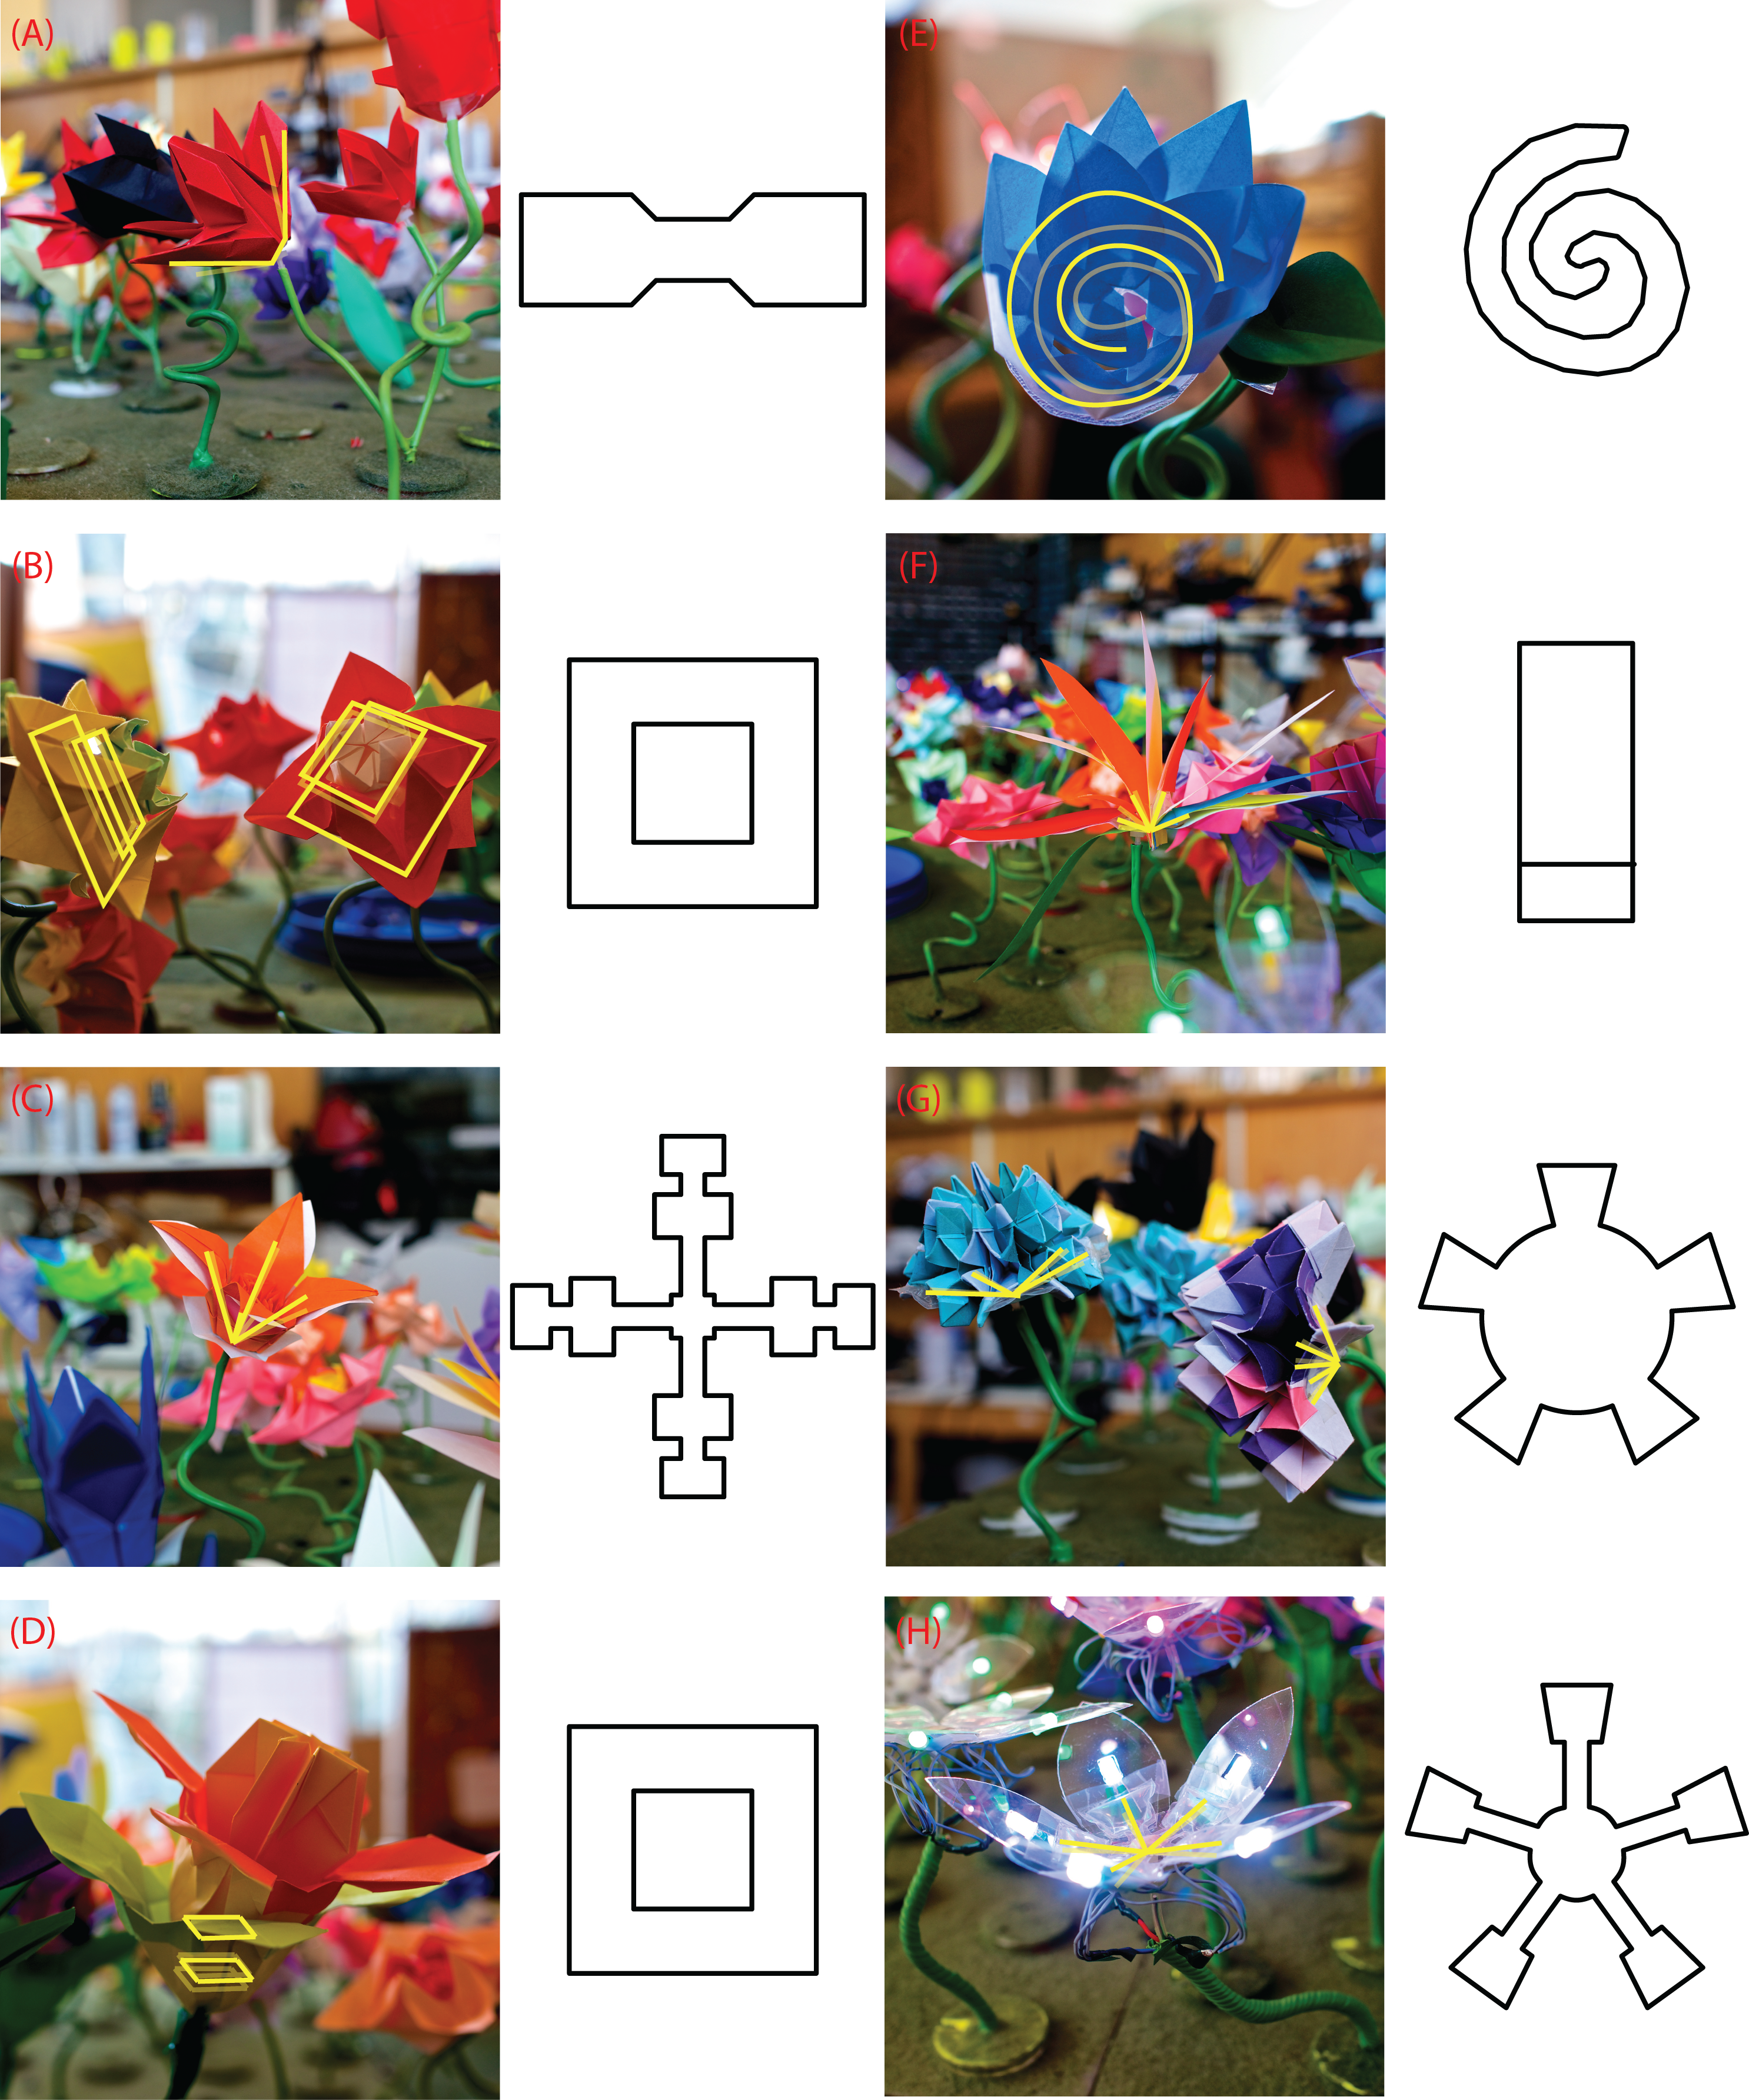
\includegraphics[scale=.22]{flowers.png}
	\caption{Pictures of inflated flowers and corresponding pouch motor designs. The locations of the pouches are marked in yellow. (A)Tulip (B) Lotus (C) Flower Lily (D) Clematis (E) Spiral Flower (F) Bird of Paradise (G) Fireworks Flower (H) LED Flower }
	\label{flowers}
\end{figure}

\section{ROBOT GARDEN CONTROL}
The computational hardware used in the garden allows each of the 16 tiles to support up to eight flowers with LEDs and pouch motors.  Each tile in the garden is controlled using an Arduino Mega2560 microcontroller equipped with additional custom boards designed to service all flower pumps and LED connections.  Each Arduino board is connected to a Bluetooth chip to allow Bluetooth communication between the tile and a computer running a Graphical User Interface developed in Python.  The PyBluez library (cite this) for Python was used for communication between the computer and the Bluetooth devices on each tile.  Additionally, the Arduino boards are connected in a wired mesh network to allow direct communication between tiles.  Algorithms have been developed for tile addressing and communication and to demonstrate distributed behaviors in the garden.


\subsection{\textbf{Computational Hardware}} 
The hardware components required for computation and control of the garden include the following for each tile: an Arduino Mega2560 board, two custom printed circuit boards, a Bluetooth chip, and wired connection to pumps, LEDs and to other Arduino boards.  In addition, a power supply is required to provide power to all Arduinos and pumps and a computer that can run Python is required for external control of the garden using the GUI.

The computational hardware used for the robot garden is extensible. The custom printed circuit boards allow the Arduino to service additional flowers and different types of flowers, so hardware can be reused if there are design changes in future versions of the garden.

\subsection{\textbf{Graphical User Interface}}
A Graphical User Interface was developed in Python so that inexperienced users can easily control the garden.  The Graphical User Interface shows the layout of the garden and has two components: the ''Control by Click'' component and the ''Control by Code'' component.  The two components of the GUI are shown in Figure~\ref{fig: GUI}.

\begin{figure}[thpb]
	\centering
	%\framebox{\parbox{3in}{hi}}
	\includegraphics[scale=0.25]{GUIComponents.png}
	\caption{Graphical User Interface (A) ''Control by Click'' component  (B) ''Control by Code'' component}
	\label{fig: GUI}
	
\end{figure}

The ''Control by Click'' component has buttons that allow the user to open and close the flowers using the pouch motors, a color wheel that allows the user to select a color for LEDs on the flowers, and buttons to turn the LEDs off and on.  Additionally there are buttons that allow users to demonstrate distributed behaviors throughout the garden.  Users can select one or multiple flowers or tiles to control and then select a command on the interface, and the selected tiles or flowers will execute the provided command.

The ''Control by Code'' component of the GUI allows users to select a flower or tile and a command from a drop-down menu.  Users then add their selected tile and command to the text using the ''Add Selection to Code'' button, and can run the commands they have chosen in sequence using the ''Run Code'' button.

\subsection{\textbf{Mesh Network and Addressing}}
Control of the garden through the GUI requires communication between a computer acting as a master device and all tiles in the garden acting as slave devices. Although each tile supports Bluetooth communication, a maximum of seven slave devices are available per Bluetooth master device (cite Bluetooth Core Specification here), so use of Bluetooth for all 16 tile connections was not possible.  As a result, we decided to establish one Bluetooth tile connection to the computer and to create a mesh network including the remaining tiles in the garden using wired serial connections for information distribution.  Each tile in the garden is a node in the mesh network and is connected to the neighboring tiles directly above, below, to the right and to the left of itself in the garden grid structure, shown in Figure~\ref{fig: Grid}.  The two center tiles were not included in the network to allow a pond or other robots to be displayed in the center of the garden.  A modified version of the  SoftwareSerial library (citation) for Arduino was used to facilitate communication between Arduino boards in the network.  
\begin{figure}[thpb]
	\centering
	%\framebox{\parbox{3in}{hi}}
	\includegraphics[scale=0.45]{GardenGridStructure.png}
	\caption{Garden Grid Structure}
	\label{fig: Grid}
	
\end{figure}


To allow tile-to-tile communication and relay of commands throughout the garden, an addressing scheme was developed so each node in the network was assigned a unique address.  Each individual tile has information about the topology of the garden mesh network, and tiles self-address accordingly.  Algorithm 1 shows the self-addressing algorithm that was used.

\begin{algorithm}
\caption{Self Addressing}\label{euclid}
\begin{algorithmic}[1]
\Procedure{Assign each tile a unique address}{}
\State $\textit{currentTile} \gets \text{address of tile running the algorithm}$\\
%\State $\textit{northNeighbor} \gets \text{tile above \textit{currentTile} in grid}$
%\State $\textit{southNeighbor} \gets \text{tile below \textit{currentTile} in grid}$
%\State $\textit{eastNeighbor} \gets \text{tile right of \textit{currentTile} in grid}$
%\State $\textit{westNeighbor} \gets \text{tile left of \textit{currentTile} in grid}$\\

\BState \emph{loop}:
\State $\text{Ping neighboring tiles for heartbeat}$
\If {$\textit{currentTile} \text{ does not have an address}$}
\If {$\text{no neighbors right or below } \textit{currentTile}$}
\State $currentTile \gets \text{Address 0}$
\Else 
\State $\text{Ping all neighbors for address of } \textit{currentTile}$
\EndIf
\Else
\State $\text{Send appropriate addresses to neighboring tiles}$

\EndIf
\EndProcedure
\end{algorithmic}
\label{fig: alg1}
\end{algorithm}

\subsection{\textbf{Arduino-to-Arduino Communication}}
When a specific flower or tile and a command are selected using the GUI, the command is routed through the Bluetooth-connected tile to the appropriate tile with minimum hops in the mesh network.  Each tile has information about the layout of the garden and can determine the next tile in the shortest path to the goal tile.  Algorithm 2 shows the command routing algorithm that was used.

\begin{algorithm}
\caption{Command Routing}\label{euclid}
\begin{algorithmic}[1]
\Procedure{Route command to correct tile and carry out command}{}
\State $\textit{serialData} \gets \text{command and goal tile data}$
\State $\textit{currentTile} \gets \text{address of tile running the algorithm}$
\State $\textit{commandTile} \gets \text{goal tile for command}$\\
%\State $\textit{myRow} \gets \text{the row of } \textit{currentTile} \text{ in grid}$
%\State $\textit{otherRow} \gets \text{row of goal tile in grid}$
%\State $\textit{northNeighbor} \gets \text{tile above \textit{currentTile} in grid}$
%\State $\textit{southNeighbor} \gets \text{tile below \textit{currentTile} in grid}$
%\State $\textit{eastNeighbor} \gets \text{tile right of \textit{currentTile} in grid}$
%\State $\textit{westNeighbor} \gets \text{tile left of \textit{currentTile} in grid}$\\

\BState \emph{loop}:
\State $\text{Listen to serial ports for incoming messages}$
\If {$\textit{serialData} \text{ received}$}
\If {$\textit{currentTile }=\textit{ commandTile} $}
\State $\text{Carry out command}$
\Else 
\If {$\textit{currentTile }\text{knows its address} $}
\State $\text{Send } \textit{serialData } \text{to next tile in shortest path}$
%\If{$\textit{myRow } = \textit{ otherRow}$}
%\If{$\textit{currentTile } < \textit{ commandTile}$}
%\State $\text{send } \textit{serialData } \text{to } \textit{westNeighbor}$
%\Else
%\State $\text{send } \textit{serialData } \text{to } \textit{eastNeighbor}$
%\EndIf
%\ElsIf{$\textit{myRow } < \textit{ otherRow}$}
%\State $\text{send } \textit{serialData } \text{to } \textit{northNeighbor}$
%\Else
%\State $\text{send } \textit{serialData } \text{to } \textit{southNeighbor}$
%\EndIf
\Else
\State $\text{Send } \textit{serialData } \text{to } \text{all neighbors}$
\EndIf
\EndIf
\EndIf
\EndProcedure
\end{algorithmic}
\label{fig: alg1}
\end{algorithm}

\subsection{\textbf{Distributed Algorithms}}
The robot garden can be used to demonstrate distributed algorithm behavior and depict graph traversal algorithms in a visually pleasing way.  Distributed behaviors are visualized by inflation and deflation of flowers on different tiles and by the changing colors of LED-lit flowers.  We implemented a flooding algorithm and a graph coloring algorithm in the garden as examples.  Two buttons in the GUI, a ''Flood'' button for the flooding algorithm and a ''Graph Coloring'' button for the graph coloring algorithm, allow users to observe the behaviors of these algorithms throughout the garden.

When the ''Flood'' button is pressed in the GUI and the flooding algorithm is called, a command is first sent to the Bluetooth-connected tile to trigger the start of the flooding behavior.  On the first tile, all flowers are inflated, and the tile sends the ''flood'' command to all of its neighbors.  When the neighbors receive the command, they inflate all of their flowers and pass the command on again.  A boolean value is used to keep track of whether or not a tile has already received a flooding command to prevent infinite looping in cycles in the garden.  After 30 seconds, enough time for the algorithm to traverse the garden, the boolean value is changed back to its original value, allowing the tile to receive the ''flood'' command if it is sent again.

When the ''Graph Coloring'' button is selected, the graph coloring algorithm is executed.  To demonstrate the graph coloring behavior, we placed at least one LED flower on each tile, so LED color on each tile and distribution throughout the garden  could easily be distinguished.  The graph coloring algorithm does this...

\section{SYSTEM PERFORMANCE}
We evaluated the performance aspects of the garden including power requirements for the whole garden, each tile, and each flower, total time required for self-addrssing, total messages sent and received per tile for self-addressing, and total time required to send a command to each tile.  The following tables show our results.

Put tables here.

What conclusions can we draw about these things...

\section{EDUCATIONAL APPLICATIONS}
The robot garden can act as a platform for art and education, particularly focused on teaching computational thinking.  The garden allows users to see their commands or code running in the physical world, linking programming to the real world.   This aspect of the garden and its colorful presentation might be especially beneficial in getting young children excited about learning to program and think computationally.  Using the garden could help young children to start thinking about the prevalence and importance of code in their daily lives.  At the same time, the garden allows children to be creative in their designs and provides them a medium for creating a new type of art using programming concepts.  

Through the ''Control by Click'' portion of the user interface, users can either control the garden directly by clicking on flowers or tiles and choosing commands or they can click on one of the algorithm visualization buttons to see algorithms demonstrated in a visual way using actuation and changing of colors of flowers in the garden.  This part of the GUI acts as a teaching tool for basic algorithm concepts.  So far, one algorithm has been demonstrated in the garden, and by leveraging the capabilities of the flower design and infrastructure of the system, many other distributed and graph traversal algorithms can be depicted in interesting ways.  

Through the ''Control by Code'' section users are able to create art using basic programming concepts.  Currently users select a tile or tiles and a command and press the ''Add to Code'' button, and they can see their commands pop up in the text box in sequential order.  Selecting ''Run Code'' runs the commands they have chosen in sequence in the garden, demonstrating basic sequential programming concepts.  In the future, we envision adding functionality to the ''Control by Code'' section that allows users to use logical statements and looping in their garden code with the aim of teaching these additional programming concepts through garden use.

In addition to adding functionality to the GUI, we plan to develop curriculum materials that leverage the capabilities of the garden to teach computational thinking.  We have already developed a versatile curriculum for middle school students that covers basic programming concepts and Finite State Machines.  This curriculum has been adapted to both Lego Mindstorms robots (cite) and the MIT SEG robot (cite) We plan to adapt the curriculum to the robot garden by adding basic sensing to the tiles and using the GUI we have already created.  In addition to using materials we already have, we will add a unit covering basic algorithms to the curriculum, making use of the visual algorithm demonstration capabilities of the garden.  Finally, we plan to invite children from local schools to use the garden and provide feedback on the garden user interface and curriculum.

\section{CONCLUSIONS}





\addtolength{\textheight}{-12cm}   % This command serves to balance the column lengths
                                  % on the last page of the document manually. It shortens
                                  % the textheight of the last page by a suitable amount.
                                  % This command does not take effect until the next page
                                  % so it should come on the page before the last. Make
                                  % sure that you do not shorten the textheight too much.

%%%%%%%%%%%%%%%%%%%%%%%%%%%%%%%%%%%%%%%%%%%%%%%%%%%%%%%%%%%%%%%%%%%%%%%%%%%%%%%%



%%%%%%%%%%%%%%%%%%%%%%%%%%%%%%%%%%%%%%%%%%%%%%%%%%%%%%%%%%%%%%%%%%%%%%%%%%%%%%%%



%%%%%%%%%%%%%%%%%%%%%%%%%%%%%%%%%%%%%%%%%%%%%%%%%%%%%%%%%%%%%%%%%%%%%%%%%%%%%%%%
\section*{APPENDIX}



\section*{ACKNOWLEDGMENT}


\begin{thebibliography}{99}

\bibitem{NiiyamaICRA2014} R. Niiyama, D. Rus, and S. Kim, ''Pouch motors: Printable/inflatable soft actuators for robotics," in \textit{Proc. of IEEE International Conference on Robotics and Automation}, 2014.
\bibitem{NiiyamaIJRR2014} R. Niiyama, X. Sun, C. Sung, B. An, D. Rus, and S. Kim, "Pouch motors: Printable soft actuators integrated with computational design," \textit{International Journal of Robotics Research}, submitted.

\end{thebibliography}
%%%%%%%%%%%%%%%%%%%%%%%%%%%%%%%%%%%%%%%%%%%%%%%%%%%%%%%%%%%%%%%%%%%%%%%%%%%%%%%%







\end{document}
